\documentclass[9pt,twocolumn,twoside,lineno]{style}

\articletype{NEI} % article type

\title{Furquim de Azevedo (1997, Capítulo 2): Níveis analíticos}
\date{13 de março de 2020}

\author[$\ddagger$]{Gabriel Petrini}
\affil[$\ddagger$]{Doutorando no instituto de Economia da Unicamp}


\runningtitle{Fichamento} % For use in the footer 

%% For the footnote.
\runningauthor{Petrini}

\begin{abstract}
	Neste capítulo, Furquim (1997) apresenta as duas principais correntes da NEI, são elas: Ambiente Institucional e Instituições de Governança. Apesar de diferentes, estes níveis analíticos tratam da importância do quadro institucional e os respectivos efeitos sobre os custos de transação (objeto). Destaca também a relevância de Williamson na consolidação da NEI e alguns conceitos. 
\end{abstract}
\keywords{}

\begin{document}

\maketitle
\articletypemark
\marginmark
\thispagestyle{firststyle}


\begin{duvidas}
	\sffamily
	\mdfdefinestyle{stylesigstyle}{linewidth=0.7pt,
		backgroundcolor=styleblueback,linecolor=stylebluetext,
		fontcolor=black,innertopmargin=6pt,innerrightmargin=6pt,
		innerbottommargin=6pt,innerleftmargin=6pt}
	{%	
		\begin{mdframed}[style=stylesigstyle]%
			\section*{Dúvidas}%
			\begin{itemize}
				\item Ao longo do capítulo são apresentadas definições de custos de transação e instituições, mas nada é dito sobre as \textbf{organizações}. Como defini-las?
				\item Quais são os fundamentos dos objetivos destacados por Davis \&
				North na citação da página 60? Não seria possível que tivessem outros objetivos que não fossem exclusivos de uma economia capitalista? Quais seriam os objetivos das instituições de uma economia não-capitalista?
				\item O que a proposição de Coase sobre a relação entre instituições e eficiência diz sobre as consequências do \textit{lock-in} (ex: QWERTY)?
			\end{itemize}
	\end{mdframed}}
\end{duvidas}



\section{Definições}
	
Apesar das diferenças, as duas principais vertentes da NEI (Ambiente institucional e Instituições de Governança) possuem elementos em comum, mais precisamente: (i) custos de transação; (ii) instituições e; (iii) organizações. Parafraseando Williamson, pontua-se:

\begin{itemize}
	\item Instituições são relevantes e suscetíveis à análise
	\item A NEI não é incompatível com a ortodoxia
	\item É multidisciplinar
\end{itemize}

\subsection{Custos de transação: O Conceito}

Nesta seção, Furquim retoma alguns temas tratados no capítulo anterior que não serão retomados neste fichamento\footnote{Coase deu uma definição muito restrita que pode ser resumida como custo de se utilizar o mercado.}. O principal a ser retido é uma definição mais precisa de custos de transação que, consequentemente, está mais sujeito à verificação empírica:
\begin{description}
	\item[Versão genérica] São custos necessários para que o sistema econômico e social funcione, ou seja, não são diretamente associados à produção e surgem na medida que os agentes interagem e \textbf{problemas de coordenação} emergem.
	\item[Definição pela negação] São todos os custos não relacionados com a transformação tecnológica de insumos em produto.
	\item[Versão mais abrangente] São custos decorrentes do uso de \textbf{qualquer forma organizacional} em que o mercado é um caso particular. Como consequência, a firma pode ser entendida como um \textbf{complexo de contratos}.
	\item[Cheung (1990)] são custos de:
		\begin{itemize}
			\item Elaboração e negociação de contratos
			\item Mensuração e fiscalização dos direitos de propriedade
			\item Monitoramento do desempenho
			\item Organização de atividades
		\end{itemize}
	Apesar de detalhada, tal definição não leva as adaptações ao ambiente econômico em consideração. Vale destacar que a \textbf{eficiência de uma governança} está associada a sua capacidade de se \textbf{adaptar} às mudanças que se dá em duas vias
		\begin{enumerate}
			\item Mudanças não antecipadas $\Rightarrow \Delta$ Transações existentes $\Rightarrow$ Revisão de contratos e de formas organizacionais $\Rightarrow$ Custos de transação
			\item Oportunidade de lucro econômico aos agentes que se adaptam mais rápido. Deficiência na adaptação $\Rightarrow$ Custos de transação $\Leftarrow$ Perda de oportunidades de lucro.
		\end{enumerate}
\end{description}
Em seguida, o autor discute o quão restrita é a qualificação de Coase dos custos de transação (memo: custos de coleta de informação e celebração de contratos). Desta discussão, vale destacar que mesmo na presença de racionalidade ilimitada e na ausência de informação assimétrica, os custos de transação continuam não sendo negligenciáveis uma vez que as informações estejam disponíveis e possam ser processadas por \textbf{todas as instâncias competentes} para a resolução de problemas contratuais. Esta constatação evidencia, por exemplo, que a regulamentação e cumprimento das regras são atividades custosas.

\subsection{Instituições}

Segue abaixo a definição de instituições de acordo com D. North (1991):

\begin{quote}
	Instituições são
	restrições (normas) construídas pelos seres humanos, que estruturam a interação social, econômica e política. Elas consistem em restrições informais e regras formais 
\end{quote}
Em seguida, Furquim destaca que as instituições não precisam ter necessariamente o propósito de restringir as interações humanas. Além disso, as instituições são os \textbf{instrumentos} adequados para as regras que compõem as instituições. Em resumo, são tanto as normas quantos os mecanismos responsáveis por sua execução.

\section{Complementaridade entre os diferentes níveis analíticos}

Além de complementares, os níveis analíticos se interagem tal como pelo esquema a seguir\footnote{Outro nível de interação que deve ser destacado é a tentativa das organizações alterarem as regras do jogo.}:

\begin{figure}[H]
	\centering
	\caption{Esquema de três níveis de Williamson (1993)}
	\label{fig:screenshot001}
	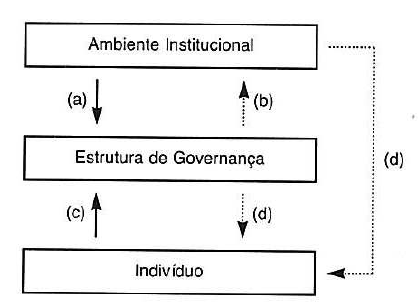
\includegraphics[width=0.4\textwidth]{figs/screenshot001}
\end{figure}


\begin{description}
	\item[Ambiente institucional] Privilegia as macroinstituições. Fornece as regras que condicionam o \textbf{aparecimento e seleção} de formas organizacionais que compõem a estrutura de governança
	\item[Instituições de governança] Enfatiza as microinstituições e se desenvolve dentro dos limites impostos pelo ambiente institucional, bem como pelos pressupostos comportamentais dos indivíduos.
\end{description}
Destaca-se ainda que ambos são mutáveis ao longo do tempo. Segue abaixo uma citação que chamou atenção:

\begin{quote}
	\textit{The institutional arrangement is an arrangement between
	economic units that govern the ways in wbich this units
	can cooperate and/or compete. It must [..] be designed to
	accomplish at least one of the \textbf{following goals}: to provide a structure within which its members \textbf{can cooperate} to obtain some \textbf{added income} that is not available outside that structure;
	or to provide a mechanism that can effect a change in laws or property rights
	designed to alter the permissible ways that individuals (or groups) can \textbf{legally compete}}
\end{quote}

Em seguida, são pontuados dois principais pressupostos \textbf{comportamentais} presentes na NEI que, por sua vez, são \textbf{necessários} para a ocorrência de custos de transação:

\begin{itemize}
	\item Os indivíduos são racionais, mas de forma limitada
	\item São oportunistas
\end{itemize}

\subsection{Ambiente Institucional}

Nesta seção, o autor destaca que a principal contribuição da corrente de \underline{Ambiente institucional} é o estabelecimento de relações entre as instituições e o \textbf{desenvolvimento econômico} destacando a importância dos \textbf{direitos de propriedade}. Além disso, destaca o reconhecimento de um \textit{trade-off} entre \textbf{especialização} e \textbf{custos de transação} (memo: especificidades dos ativos discutidas no capítulo anterior). O papel das instituições seria conciliar esse movimento antagônico, ou seja, \textbf{impedir o aumento dos custos de transação na medida que a especialização aumenta}. Dito isso, o autor detecta dois caminhos dessa corrente:
\begin{enumerate}
	\item Investigar os efeitos de uma mudança no ambiente institucional sobre o resultado econômico
	 \item teorizar sobre a criação das instituições
\end{enumerate}
Em seguida, discute alguns trabalhos dessa corrente, enfatizando a endogeinização das instituições que, como consequência, compromete encará-las como um fatos determinante (como pontua a NEI).

\subsection{Economia dos Custos de Transação:a análise da estrutura de governança}

Em linhas gerais, esta corrente toma as regras do jogo como dadas e fornece os microfundamentos para o estudo do ambiente institucional que, por sua vez, fornece os parâmetros para a ECT. Tem na redução dos custos de transação sua principal função.

\section{Instituições e eficiência}

A compreensão da relação entre instituições e eficiente parte da proposição a seguir:

\begin{description}
	\item[Proposição de Coase] As instituições mais eficientes são aquelas efetivamente adotadas.
\end{description}
Furquim pontua que boa parte dos trabalhos empíricos buscaram testá-la. Por fim, vale destacar o paradoxo entre formas organizacionais eficientes e insignificância das instituições dada subsequente redução dos custos de transação:
\begin{description}
	\item[Paradoxo da NEI:] a escolha das instituições somente será eficiente
	se custos de transação forem negligenciáveis; porém, se isso for verdadeiro, então a escolha de instituições é irrelevante, uma vez
	que sua relevância decorre da presença de custos de transação.  
\end{description}
	
% Please add here a significance statement to explain the relevance of your work
%\afterpage{
\begin{sigstatement}
	\sffamily
	\mdfdefinestyle{stylesigstyle}{linewidth=0.7pt,
		backgroundcolor=styleblueback,linecolor=stylebluetext,
		fontcolor=stylebluetext,innertopmargin=6pt,innerrightmargin=6pt,
		innerbottommargin=6pt,innerleftmargin=6pt}
	{%	
		\begin{mdframed}[style=stylesigstyle]%
			\section*{5 Seconds Synthesis}%
			\lipsum[1]
	\end{mdframed}}
\end{sigstatement}
%}



	
\end{document}